\documentclass{article}
\usepackage{iclr2027_conference,times}
\usepackage{graphicx,booktabs,amsmath,amssymb}
\usepackage{hyperref,url}
\title{Benchmark scores after prompt selection:\\Accuracy, uncertainty, and reporting costs}
\author{Anonymous authors}
\begin{document}
\maketitle
\begin{abstract}
Selecting a configuration and reporting its score on the same questions can conflate accuracy with favorable sampling noise. We distinguish selected-system accuracy, selection quality, and reporting calibration, comparing reused scores, simultaneous fixed-bank intervals, and independent auditing. In 288 controlled settings with 20,000 repetitions each, optimism and decision errors depend strongly on sample size, bank size, dependence, and quality separation. Newly generated Qwen2.5-1.5B responses on MMLU-Pro give a frozen winner 36.72\% reused accuracy versus 25.39\% disjoint-audit accuracy, a gap of 11.33 percentage points with adjusted exact interval [6.85,15.45]. The default also has a sizable gap, so the full difference is not attributable solely to selection. Known-truth resampling of the real response cache finds positive bias but no observed nominal interval undercoverage in this small bank. Auditing and simultaneous protection address different reporting failures, with distinct uncertainty, selection-quality and inference-cost tradeoffs. Reliable reports must name their selected target, search exposure, sampling design and reporting budget.
\end{abstract}
\section{Introduction}
A benchmark score is interpretable only together with the procedure that produced the evaluated system. If a search evaluates many prompts on the same questions and returns the empirical winner, the winning score reflects both performance and favorable sampling noise. Reporting that score as if the prompt had been fixed before evaluation can distort uncertainty and subsequent comparisons. The relevant question is quantitative: how much distortion occurs under a specified search, and what resources are needed for a more reliable report?

We study exhaustive automated selection from a frozen bank of configurations. This restricted setting separates selection from candidate generation: the bank exists before evaluation outcomes are observed. It is an authentic search procedure, but it does not represent every compiler that constructs instructions, demonstrations, or pipelines using feedback. In particular, our fixed-bank guarantees do not extend merely by counting the prompts produced by an adaptive generator.

Our central target is the fresh-question accuracy of the configuration actually chosen by the search. This differs from the best available configuration's accuracy and from average quality over repeated searches. These distinctions determine whether an interval, a holdout estimate, and a claim of improvement answer the same question. A reporting correction can improve calibration without improving the chosen system, while reserving evaluation questions can change which system is chosen.

The underlying selection effect and its standard remedies have established statistical foundations. Our contribution is an empirical assessment that connects their assumptions, calibration, decision consequences, and resource costs in a precisely specified configuration-search setting. Controlled experiments isolate sample size, bank size, shared errors, and quality differences. We compare reused-score reporting, simultaneous fixed-bank intervals, and independent auditing, including splits that preserve either total questions or total model calls. We distinguish their targets and report uncertainty from repeated whole-search experiments.

Our real-model study uses newly generated responses on MMLU-Pro and separates three kinds of evidence: a disjoint audit for the selected system on the remaining benchmark, conditional reselection on one response matrix, and reporting calibration against known empirical-cache truth. They support different claims. The real setting exhibits a substantial reuse--audit gap and an audit-supported improvement over default, but does not reproduce the synthetic large-bank undercoverage. This combination motivates reporting the setting and target rather than assuming that every optimized score has the same failure.

\section{Related work}
\paragraph{Optimizing language-model configurations.}
DSPy compiles declarative language-model programs using metric-driven optimization \citep{khattab2023dspy}; MIPRO jointly optimizes instructions and demonstrations \citep{opsahlong2024mipro}. Their evaluation protocols distinguish development and final evaluation data. Our reuse protocol is a specific statistical risk, not a claim that these tools necessarily evaluate incorrectly. Best-arm identification emphasizes selecting good prompts under a fixed evaluation budget \citep{shi2024bestarm}. Selection quality and the accuracy of a reported winning score remain different objectives.

\paragraph{Variation across prompts.}
FormatSpread studies performance ranges over formatting choices \citep{sclar2023formats}; PromptEval estimates distributions and quantiles of prompt performance from sparse evaluations \citep{polo2024multiprompt}. A range or performance quantile across prompts is not a confidence interval for a chosen prompt's fresh-question accuracy. We retain this distinction when comparing genuine quality differences with sampling optimism. MMLU-Pro supplies a more challenging, multidisciplinary benchmark and studies prompt robustness \citep{wang2024mmlupro}; robustness in a benchmark study does not itself establish post-selection calibration.

\paragraph{Selection and data reuse.}
Overfitting a noisy model-selection criterion and evaluating after selection are classical problems \citep{cawleytalbot2010selection}. Inference on winners explicitly distinguishes the population quality of the observed winner from the population maximum, and marginal from identity-conditional validity \citep{andrews2021winners}. Simultaneous protection before arbitrary selection within a specified family is an established principle \citep{berk2013posi}; we use elementary binomial intervals rather than importing regression-specific guarantees. Adaptive data analysis and Ladder instead protect controlled feedback interactions \citep{dwork2014adaptive,blumhardt2015ladder}. We do not implement those mechanisms or claim their guarantees after unrestricted label access. Independent auditing, splitting, and multiplicity correction are established tools; this study assesses their behavior and costs rather than claiming their invention. The permitted literature is deliberately scoped, so we make no claim of an exhaustive novelty search.

\section{Targets and reporting protocols}
\label{sec:methods}
\subsection{What does a selected score estimate?}
Let $j\in\{0,\ldots,K-1\}$ index a configuration fixed independently of the evaluation questions. A configuration includes the model, prompt, decoding, and scoring rule. For a question $X\sim P$, let $Y_j(X)\in\{0,1\}$ denote correctness and $\theta_j=\mathbb{E}_P Y_j(X)$ its accuracy. Scores for different configurations on the same question can be arbitrarily dependent. For the controlled and empirical-cache experiments below, search questions $S=(X_1,\ldots,X_n)$ are iid from the specified distribution, and exhaustive search returns
\begin{equation}
 \hat j=\arg\max_j\hat\theta_{Sj},\qquad
 \hat\theta_{Sj}=\frac1n\sum_{i=1}^nY_j(X_i),
\end{equation}
with independent uniform tie breaking. The reused report is $R=\hat\theta_{S\hat j}$, and its realized error is $R-\theta_{\hat j}$. Expected optimism averages this error over complete reruns of search. The selected target $\theta_{\hat j}$ is distinct from procedure quality $\mathbb{E}_S\theta_{\hat j}$ and the oracle $\max_j\theta_j$. A positive realized error is not guaranteed on every run.

For a fixed bank and iid bounded scores,
\begin{equation}
 0\leq\mathbb{E}[R-\theta_{\hat j}]
 \leq\sqrt{\frac{\log K}{2n}}.
 \label{eq:optimism}
\end{equation}
The lower bound follows from $\mathbb{E}\max_j\hat\theta_{Sj}\geq\max_j\theta_j\geq\mathbb{E}\theta_{\hat j}$. A bounded moment-generating-function argument gives the upper bound (Appendix~\ref{app:guarantees}). This expectation bound is often loose, particularly with strongly shared errors. It does not imply that optimization cannot improve true quality.

\subsection{Reporting alternatives}
\paragraph{Reuse.}
Report the winning search accuracy with its ordinary two-sided 95\% Clopper--Pearson (CP) interval. CP has a fixed-candidate binomial guarantee; selecting the candidate using the same outcomes does not preserve that guarantee.

\paragraph{Simultaneous fixed-bank protection.}
Construct CP intervals for every candidate at marginal error $0.05/K$, then report the interval for $\hat j$. A union bound gives simultaneous coverage at least 95\%, hence at least 95\% coverage for the selected member, without independence across candidates. This changes the interval, not the reused point estimate. The guarantee requires an outcome-independent family; unrestricted feedback-based creation of new candidates is a different problem.

\paragraph{Independent audit.}
Freeze the selected configuration before evaluating it on $h$ iid fresh questions. The audit score is conditionally unbiased for $\theta_{\hat j}$, with variance $\theta_{\hat j}(1-\theta_{\hat j})/h$ and ordinary CP coverage at least 95\%. Further selection after viewing audit outcomes would change the argument. We compare an additional audit of size $n$ after full search with two split protocols. A question split reserves $h=n-\lfloor n/2\rfloor$ questions and searches on $s=\lfloor n/2\rfloor$, preserving $n$ total question draws. A call split takes
\begin{equation}
 s=\left\lfloor\frac{nK}{K+1}\right\rfloor,\qquad h=nK-sK,
\end{equation}
so $sK+h=nK$ preserves total scoring calls. The latter can use more question draws. Both splits can select a different configuration from full search; their reports target their own winners.

\subsection{How reliability is evaluated}
We rerun selection in each repetition and measure signed error, mean squared error (MSE), interval coverage and width, and selected true quality. All intervals concern the selected configuration's accuracy, with marginal coverage over the random selected identity. We do not claim identity-conditional coverage from a marginal result.

For a concrete decision endpoint, candidate 0 is a frozen default. Declare superiority when a nondefault winner's ordinary 95\% CP lower endpoint exceeds the default's corresponding upper endpoint. A false claim has $\theta_{\hat j}\leq\theta_0$. The two relevant one-sided errors sum to at most 0.05 for a frozen pair; that argument need not hold after choosing the pair by search. We also evaluate the simultaneous-interval version. We report unconditional false-superiority frequency, not the fraction of claims that are false, and do not identify this interval-nonoverlap rule with a paired test.


\subsection{Finite-benchmark and empirical-cache targets}
The primary real-benchmark protocol uses sampling without replacement rather than the iid experiment above. A prespecified runtime fallback retains four candidates, 256 search questions and 512 disjoint audit questions from the pinned MMLU-Pro benchmark's 12,032 test items. Conditional on the retained search reservoir $S_C$, the target for a chosen configuration is its question-weighted accuracy on the remaining 11,776 items, $\theta_{\rm rem}(\hat j;S_C)$. Smaller search subsets retain this same complement target. The audit score carries sampling uncertainty and is not known truth.

For each fixed design, exact hypergeometric inversion supplies audit intervals and transformed simultaneous-search intervals for this target. However, runtime can depend on item properties related to correctness. Outcome-blind choice between the original and fallback designs therefore does not by itself preserve fixed-design guarantees conditional on that choice. The supplied analysis allocates error $0.05/2$ to each possible design, with a further bank adjustment where needed. A union bound protects the runtime-chosen interval at least 95\% unconditionally over partition and tier choice, separately for each endpoint family. We claim neither coverage nor audit unbiasedness conditional on the runtime trigger, nor joint protection of all reported endpoints. Appendix~\ref{app:real-protocol} gives the sampling argument, transformation, scope history and costs.

A separate calibration experiment samples whole paired rows iid with replacement from the 768-row retained response cache, rerunning selection and reporting. Candidate means in that empirical distribution are known, permitting coverage and decision error to be measured against its conditional truth with the original 95\% iid protocols. This does not establish calibration on the unobserved remainder of the benchmark. Reusing one audit pool likewise cannot remove its sampling uncertainty by increasing the number of Monte Carlo repetitions.

\section{Controlled experiments}
\label{sec:synthetic}
\subsection{Design and validation}
The synthetic experiment has known candidate accuracies, allowing genuine coverage and decision error to be measured. Candidate 0 has accuracy 0.4. Equal-quality cells set every candidate to 0.4; heterogeneous cells place the other candidates evenly over $[0.32,0.48]$ ($K=2$ has a single challenger at 0.48). On each independent question, with probability $\rho$ all candidates compare a shared $U\sim\mathrm{Uniform}(0,1)$ against their own accuracy; otherwise they compare independent uniforms. Thus
\begin{equation}
 \mathrm{Cov}(Y_j,Y_k)=\rho\{\min(\theta_j,\theta_k)-\theta_j\theta_k\},\quad j\ne k.
\end{equation}
Each marginal variance is $\theta_j(1-\theta_j)$, independently of $\rho$. For equal accuracies, pairwise correctness correlation equals $\rho$; for heterogeneous accuracies, $\rho$ is the mixture probability rather than the correlation itself.

The complete grid crosses $n\in\{16,32,64,128,256,512\}$, $K\in\{1,2,4,8,16,32,64,128\}$, $\rho\in\{0,0.5,0.9\}$, and quality-spread parameter $\{0,0.08\}$. Each of 288 cells has 20,000 independent repetitions, for 5.76 million whole-search experiments, with master seed 20261103. Each reported mean has a Monte Carlo standard error (MCSE); for rates the standard error is computed across independent event indicators. These uncertainties concern simulation error. All outcomes, including no-selection and small-gap cases, are retained.

An exact sufficient-count sampler avoids materializing every binary row while preserving the specified joint law. Distributional checks compare means and covariances with analytic values and test dependence endpoints. Exact binomial-maximum calculations independently check optimism, naive coverage, and simultaneous coverage in 48 independent equal-quality settings. Across 144 checks, the largest absolute simulation discrepancy is 3.651 MCSE. This validates the implementation against these references; it is not a universal proof of software correctness.

\subsection{Magnitude and drivers of score optimism}
Figure~\ref{fig:selection} isolates selection without genuine improvements: all candidates have accuracy 0.4. At $n=64$, $K=16$, and $\rho=0.5$, reuse overstates the selected accuracy by 7.705 percentage points on average (MCSE 0.035 pp). The ordinary nominal 95\% interval covers only 82.295\% of selected targets (MCSE 0.270 pp). Increasing the question count reduces sampling noise; increasing the bank size supplies more opportunities to select favorable noise. Shared errors reduce the effective diversity of these opportunities. These are conditional patterns under the specified data-generating mechanism, not a universal formula for real prompts.

The complete grid includes favorable cases as well as severe failures (Appendix~\ref{app:fullgrid}). At $n=512$, $K=128$, $\rho=0.9$, and spread 0.08, reused-score optimism is 1.031 pp (MCSE 0.015 pp). A clear quality advantage and strongly shared errors can therefore substantially reduce optimism. Across the prespecified grid, naive selected-candidate coverage ranges from 5.165\% to 97.525\%; these are empirical extrema, not simultaneous confidence limits for population extrema. In heterogeneous cells, changing $K$ also changes the true-quality grid, so the equal-quality cells provide the clean comparison for bank-size effects.

\begin{figure}[t]
\centering
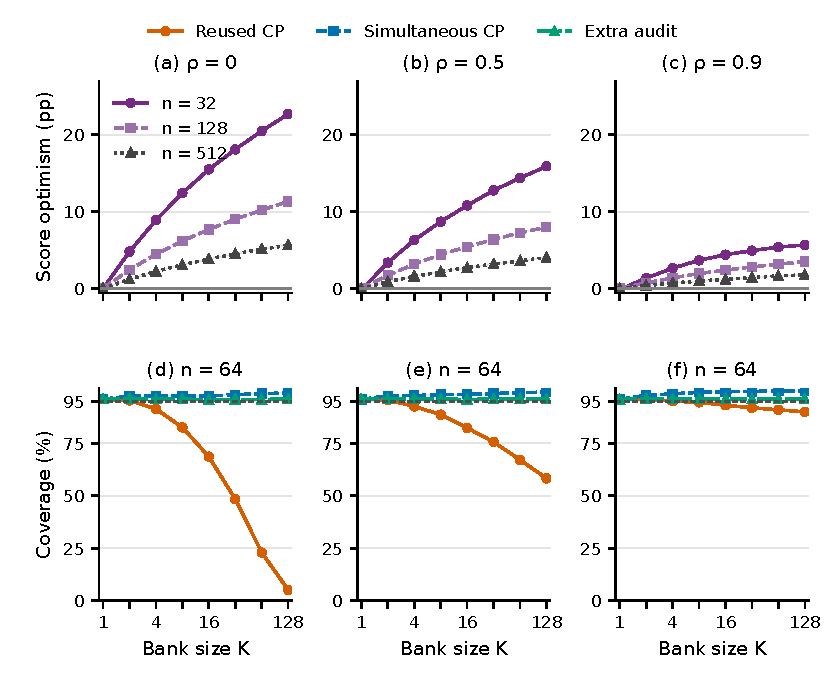
\includegraphics[width=\linewidth]{figures/synthetic-selection.pdf}
\caption{\textbf{Selection optimism and interval validity depend on bank size and shared errors.} All candidates have true accuracy 0.4. Columns vary correctness correlation $\rho$. Top: mean winning search score minus truth, for the labeled iid question counts $n$. Bottom: selected-target coverage of nominal 95\% CP intervals at $n=64$; the gray line marks 95\%. Simultaneous CP uses marginal error $0.05/K$. Extra audit scores the full-search winner on $n$ additional independent questions, costing $n$ calls beyond $nK$ search calls. Bands are marginal 95\% Monte Carlo intervals: mean $\pm1.96$ MCSE for optimism and exact binomial intervals for coverage, with 20,000 repetitions per cell. Some bands are narrower than markers. Correcting an interval leaves the reused point score unchanged.}
\label{fig:selection}
\end{figure}

\subsection{Reliability, utility, and resource costs}
Appendix Table~\ref{tab:methods} illustrates two declared settings. In the equal-quality case, simultaneous coverage is 98.290\% (MCSE 0.092 pp), and an extra independent audit gives 95.835\% (MCSE 0.141 pp). Over the grid, their coverage estimates range from 95.145\% to 99.955\% and from 95.065\% to 97.605\%, respectively. CP discreteness and simultaneous correction both contribute conservatism; measured minima do not establish a simultaneous empirical guarantee. The mathematical guarantees depend on the fixed-bank iid assumptions in Section~\ref{sec:methods}.



Reliable intervals need not be equally informative or equally costly (Appendix Figure~\ref{fig:budgets}). Simultaneous intervals avoid extra inference calls but widen. Extra auditing retains full-search quality and pays for additional observations. Reserving half the questions changes both the search winner and audit precision. At $n=128$, $K=32$, $\rho=0.5$, and spread 0.08, full search selects true quality 46.52\% (MCSE 0.011 pp), whereas the equal-question split selects 45.85\% (MCSE 0.016 pp). Its wider intervals and lower selected quality must be considered alongside its calibration. The call split spends fewer evaluations on every candidate to free calls for auditing only the winner; it permits more question draws than the question split. No method dominates all these criteria. Appendix~\ref{app:mse} reports MSE, which simultaneous intervals cannot change because they preserve the point score.



\subsection{Consequences for a reported comparison}
Even the conservative interval-nonoverlap decision can fail after selection. At $n=512$, $K=128$, and independent equal-quality candidates, false superiority is reported in 9.890\% of repetitions (MCSE 0.211 pp), despite there being no true improvement. The frozen-pair 5\% error argument does not protect the data-selected pair. Appendix~\ref{app:decisions} shows the dependence on $K$ and $\rho$ and the simultaneous-interval comparison. This is evidence about this explicit decision rule, not a general false-discovery rate. Zero observed events in 20,000 repetitions would still permit a one-sided 95\% upper risk of approximately 0.015\%.

\section{Newly generated real-model evidence}
\label{sec:real}
\subsection{Frozen search and fresh-question audit}
We newly generated Qwen2.5-1.5B-Instruct Q4\_K\_M answers on pinned MMLU-Pro, using greedy CPU inference and a strict, frozen capital-letter parser. The benchmark has 12,032 test questions in 14 categories, with 3--10 options. Validation questions checked implementation and timing. Neither gold answers nor rationales entered generation. Four instruction/format candidates, including default 0, were searched on 256 questions; 512 disjoint questions provide the audit. The primary matrix contains 3,072 answers. An outcome-blind, prespecified calendar rule reduced the original design after a completed eight-candidate shard; all 6,144 generated answers are preserved and costed. Appendix~\ref{app:real-protocol} records the freeze, fallback, exact inference and compute. The target is the 11,776-question complement defined in Section~\ref{sec:methods}, not full-benchmark or unrestricted future-task accuracy.

Figure~\ref{fig:real-primary} shows the unique search winner, candidate 10: 94/256, or 36.72\%, compared with 130/512, or 25.39\%, on audit. Its adjusted exact audit interval is [21.27,29.87]\%; the observed reuse--audit gap is 11.33 pp, with interval [6.85,15.45] pp for reused score minus remaining-benchmark accuracy. The transformed simultaneous-search interval for remaining-benchmark accuracy is [28.55,45.46]\%. These finite-population intervals have the two-design unconditional guarantees specified above, separately per endpoint family; one realization cannot measure coverage.

Crucially, default 0 also drops from 25.39\% search to 16.80\% audit, a gap of 8.59 pp. The winner's excess gap beyond that default gap is only 2.73 pp, with adjusted interval [$-2.81$,8.45] pp. Thus the entire 11.33 pp cannot be identified as selection-only optimism. A single partition does not distinguish sampling variation, optimization, or other explanations of the common gap.

The winner improves over default on paired audit questions: 61 wins and 17 losses give +8.59 pp, with adjusted exact paired interval [2.88,14.14] pp. The conservative ordinary reused-interval nonoverlap rule does \emph{not} declare superiority; the adjusted audit nonoverlap rule does, and the paired audit lower bound is positive. Reporting changes the decision toward audit-supported improvement here. This is not an observed false-positive reuse decision, nor an estimate of population false-superiority risk.


\begin{figure}[t]
\centering
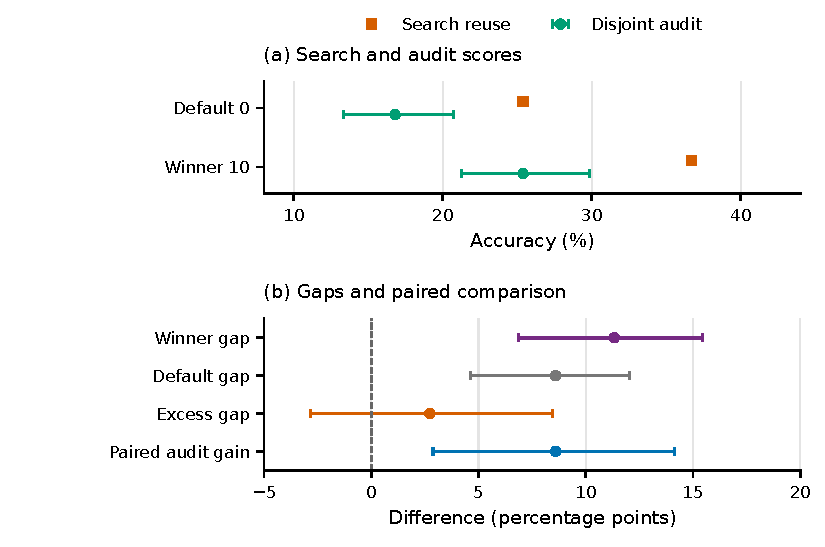
\includegraphics[width=\linewidth]{figures/real-primary.pdf}
\caption{\textbf{The default shares much of the winner's search--audit gap.} Qwen 2.5-1.5B-Instruct on MMLU-Pro; four frozen candidates, 256 search and 512 disjoint audit questions. (a) Squares: search scores; circles: audit estimates of accuracy on the 11,776-question reservoir complement. (b) Search-minus-audit gaps, their difference (excess gap), and paired winner-minus-default audit gain. The winner gap is 11.33 pp versus the default's 8.59 pp; the excess-gap interval crosses zero, so the full gap cannot be identified as selection-only optimism. Whiskers use exact finite-population endpoints with error .025 per possible runtime design: at least 95\% unconditional protection separately per endpoint family, without a joint-all-endpoint or conditional-on-trigger guarantee. This is one realized partition. The paired gain supports improvement; the primary reporting/decision/cost table gives the distinct comparison rules.}
\label{fig:real-primary}
\end{figure}

\subsection{Reselection and reporting calibration}
We repeat selection 20,000 times in each of 15 $n/K$ cells, $n\in\{16,32,64,128,256\}$ and $K\in\{1,2,4\}$, conditional on the same search/audit matrices. At $K=4$, mean reuse--audit gaps are 14.59, 11.55 and 11.33 pp for $n=16,64,256$; $K=1$ retains the default's approximately 8.59 pp gap. MCSE describes conditional computation, not fresh-pool uncertainty. A paired-row bootstrap independently resamples both pools and reruns selection (1,000 outer, 2,000 inner repetitions). Its approximate 95\% sensitivity range for the gap at $n=256,K=4$ is [4.69,18.55] pp. These ranges do not replace exact audit uncertainty or supply runtime-conditional coverage.

For a separate known-truth experiment, we sample whole rows iid with replacement from the retained 768-question/four-candidate cache. The selected candidate's exact cache mean is the target. Figure~\ref{fig:real-cache} summarizes calibration; 20,000 repetitions per cell evaluate all five reporting protocols from Section~\ref{sec:methods}. At $K=4$, reuse optimism decreases from 4.97 pp (MCSE 0.075) at $n=16$ to 0.214 pp (MCSE 0.020) at $n=256$.

Ordinary nominal 95\% coverage across all 15 cells is \mbox{95.290--97.585\%}: this small real bank exhibits positive point bias \emph{without observed nominal undercoverage}. It does not reproduce the large-bank synthetic coverage failure.

At $n=256,K=4$, ordinary, simultaneous and independent-audit coverage is 95.425\%, 98.905\% and 95.510\%, with mean widths 11.46, 14.46 and 11.43 pp. Simultaneous protection is conservative and widens without changing point bias. Full-search selected cache quality is 29.02\%, compared with 28.75\% under half-question splitting and 28.94\% under equal-call splitting; these are their respective winners' qualities. Reuse uses 1,024 logical calls, extra auditing 1,280, question splitting 640, and call splitting 1,024. These calibration budgets differ from the primary disjoint audit and actual generation costs. The largest per-cell false-superiority frequency is one in 20,000 (naive reuse); zero events still allow a per-cell one-sided 95\% upper risk of 0.015\%.


\begin{figure}[t]
\centering
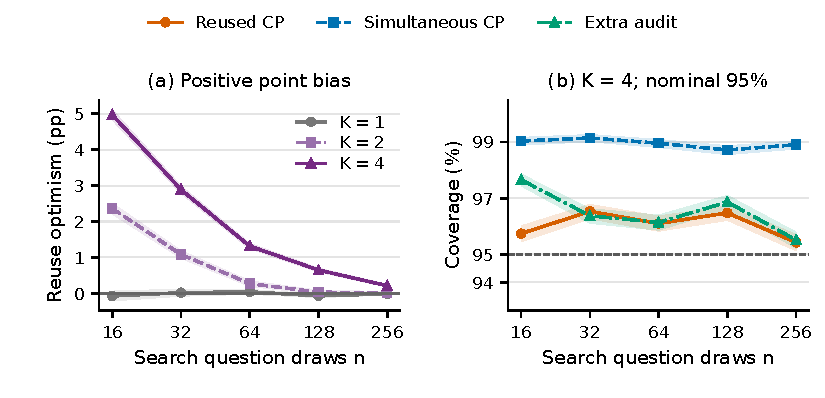
\includegraphics[width=\linewidth]{figures/real-cache-main.pdf}
\caption{\textbf{Positive point bias coexists with no observed nominal undercoverage in this small bank.} Whole paired rows from the 768-question/four-candidate cache are drawn iid with replacement; full selection/reporting is repeated 20,000 times per cell. Truth is the selected candidate's exact empirical-cache mean. (a) Reuse optimism by frozen-prefix bank size K. (b) Coverage of nominal 95\% Clopper--Pearson (CP) reporting at K=4; dashed line: 95\%. Bands are marginal 95\% computational intervals (mean $\pm$ 1.96 MCSE for optimism, exact binomial for coverage), conditional on this cache. Reuse coverage is 95.290--97.585\% across all 15 cells. This calibration target differs from remaining-benchmark accuracy in the primary display. Simultaneous CP keeps the reused point score; extra audit uses n additional question draws/calls. Full five-method coverage, widths, selection quality, score error, decisions and budgets accompany the appendix.}
\label{fig:real-cache}
\end{figure}

\paragraph{Diagnostics and scope.}
The retained responses include 398 malformed answers (12.96\%) and no out-of-range letters. Winner 10 has none; default 0 has 164/768. Format adherence is part of the measured system, so improvements cannot be interpreted purely as knowledge gains. All contexts fit. Candidate correctness correlations span 0.531--0.699; this descriptive range does not identify a causal dependence effect. Category results retain explicit denominators and question weighting. All raw responses, complete driver/calibration grids, uncertainty, diagnostics and costs accompany the code.

Appendix~\ref{app:real-evidence} gives the full grids, numerical decision/cost comparisons, sensitivity ranges and diagnostics.

\section{Discussion and limitations}
A report should identify the selected configuration, the information exposed during search, and the questions supporting its score. For an outcome-independent bank, simultaneous intervals acknowledge selection without extra calls but retain point optimism. Independent auditing evaluates the frozen winner; splitting can change that winner. Selection/report sample sizes, candidate bank and tie rule, interval construction, and question-draw versus inference-call costs are therefore part of the reported result.

The evidence is conditional on setting. Synthetic equal-quality, diverse banks exhibit severe coverage and decision failures; shared errors and quality separation can reduce them. The real experiment shows a large reuse--audit difference and a positive paired audit effect, while its known-cache calibration finds positive bias without nominal undercoverage. The default's gap prevents attributing the full observed winner gap to selection. Neither a severe synthetic cell nor a favorable small real bank establishes a universal magnitude or universal safety.

Our exhaustive frozen-bank search does not study feedback-driven prompt creation or multi-call pipeline optimization. The synthetic mixture captures only some dependence structures; heterogeneous bank size also changes available qualities. The real evidence concerns one small quantized direct-answer model, one benchmark partition, a strict parser, and a reduced four-candidate design. Format failures contribute to performance differences, and possible benchmark contamination during pretraining is not measured. Larger models, richer decoding, other tasks and adaptive generators require new evidence.

The disjoint audit estimates remaining-benchmark accuracy. The two-design correction protects endpoints unconditionally and separately by family; it gives no trigger-conditional coverage or unbiasedness. Cache resampling reruns selection and targets known empirical means, without repeating LLM generation. Bootstrap sensitivity and conditional MCSE do not establish external-population coverage. Our conservative comparison is one policy; zero observed errors do not establish zero risk.

\clearpage
\label{post-main-start}
\section*{AI use statement}
This study is conducted by an AI research-agent workflow. AI agents developed the questions and design, mathematical exposition and checks, synthetic generator, experiment and inference code, analyses, figures, literature notes, manuscript text, and revisions. Separate roles supply context, planning, feasibility assessment, analysis, presentation, venue requirements, manuscript integration, and internal and external review. These separations provide checks within the workflow; they are not independent human verification. Completed checks include distributional tests, exact-null and finite-population references, parser and partition checks, raw-output/source provenance, numerical manuscript checks, compilation, and visual inspection. The experimental language model is distinct from the agents conducting the research. No human audit, author consensus, or conference acceptance is asserted.

\section*{Ethics statement}
The study uses synthetic binary outcomes and a public knowledge benchmark. Its principal research-integrity concern is overstating the meaning of a selected score or an uncertain audit. We preserve negative findings, scope limits, source versions, raw outputs and failures. A benchmark score does not establish suitability for consequential deployment. We do not claim that prompt optimizers inherently misuse evaluation data or that one model's results generalize to all models. Dataset/model license and acquisition records accompany the reproduction package.

\section*{Reproducibility statement}
The supplied repository contains the LaTeX source/PDF, pinned official template, analysis and presentation code, all generated responses, scoring matrices, complete numerical results and source hashes. Its README gives environment, acquisition, validation, generation, cached-analysis, rendering and build entry points. The appendix specifies selected targets, sampling, frozen search and parser, seeds, uncertainty, scope changes, measured compute and failures. Cached reproduction does not require new inference; repeating generation requires the separately documented native backend and pinned public weights.

\bibliographystyle{iclr2027_conference}
\bibliography{references}
\clearpage
\appendix
\section{Guarantees and their scope}
\label{app:guarantees}
For completeness, the fixed-bank expectation bound in Equation~\eqref{eq:optimism} follows from a bounded-score argument. Write $M_j=\hat\theta_{Sj}$. Since $M_{\hat j}=\max_jM_j$,
\begin{align}
\mathbb{E}(M_{\hat j}-\theta_{\hat j})
&=\mathbb{E}\max_jM_j-\mathbb{E}\theta_{\hat j}\\
&\geq\max_j\theta_j-\mathbb{E}\theta_{\hat j}\geq0.
\end{align}
For $\lambda>0$, iid bounded observations imply
$\mathbb{E}e^{\lambda(M_j-\theta_j)}\leq e^{\lambda^2/(8n)}$. Therefore
\begin{align}
\mathbb{E}(M_{\hat j}-\theta_{\hat j})
&\leq\mathbb{E}\max_j(M_j-\theta_j)\\
&\leq\frac{\log K}{\lambda}+\frac{\lambda}{8n}.
\end{align}
Optimizing $\lambda$ yields the upper bound for $K>1$; for $K=1$ unbiasedness is immediate. Independence across configurations is unnecessary, while independence across question rows and a fixed family are essential to this argument.

If $C_j$ is a CP interval with marginal error $\alpha/K$, then
\begin{equation}
\Pr(\forall j:\theta_j\in C_j)\geq1-\sum_j\alpha/K=1-\alpha.
\end{equation}
Thus $\Pr(\theta_{\hat j}\in C_{\hat j})\geq1-\alpha$ for any selector within the protected family. On this simultaneous event, the winner cannot have a lower interval endpoint exceeding the default's upper endpoint when its true accuracy is no greater than the default's. This protects the specified simultaneous-interval comparison. It does not make the reused point estimate unbiased.

For a fresh independent audit of a frozen winner, conditional on the entire search dataset and its randomization, the audit count is $\mathrm{Binomial}(h,\theta_{\hat j})$. Conditional unbiasedness and CP coverage follow, and remain valid on averaging over search. The simple proof ceases to apply if audit outcomes guide further configuration changes. For a finite scored cache, iid resampling with replacement gives a conditional empirical-population target; that target is not automatically the unknown superpopulation accuracy. Our synthetic experiments use genuinely known Bernoulli parameters.

\clearpage
\section{Decision errors under selection}
\label{app:decisions}
\begin{figure}[htbp]
\centering
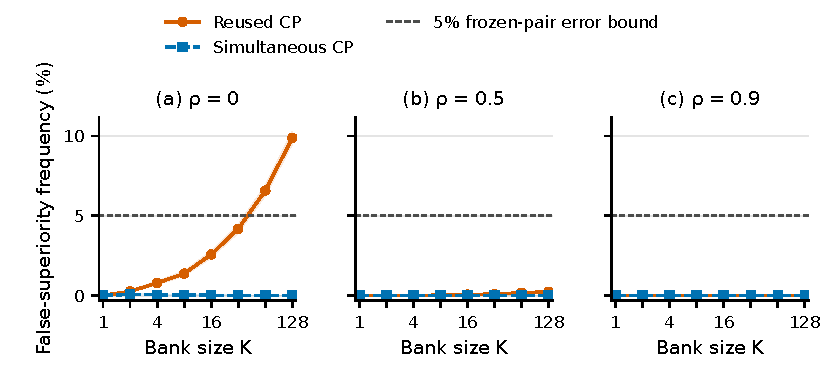
\includegraphics[width=\linewidth]{figures/synthetic-decisions.pdf}
\caption{\textbf{A conservative frozen-pair rule can become unreliable after winner selection.} At $n=512$, every candidate has accuracy 0.4. An event occurs when a selected nondefault winner's lower ordinary 95\% CP endpoint exceeds the default's upper endpoint. Rates are unconditional over all repetitions, not conditional false-discovery rates. The dashed 5\% line is the frozen-pair bound before selection. Simultaneous CP uses per-candidate error $0.05/K$. Columns vary equal-quality correlation $\rho$; bands are marginal exact 95\% binomial Monte Carlo intervals over 20,000 repetitions. At $\rho=0$, $K=128$, the ordinary-rule rate is 9.89\% (MCSE 0.211 pp). Zero events would not establish zero population risk. This rule is not a paired test.}
\end{figure}

\clearpage
\section{Complete synthetic grid}
\label{app:fullgrid}
\begin{figure}[htbp]
\centering
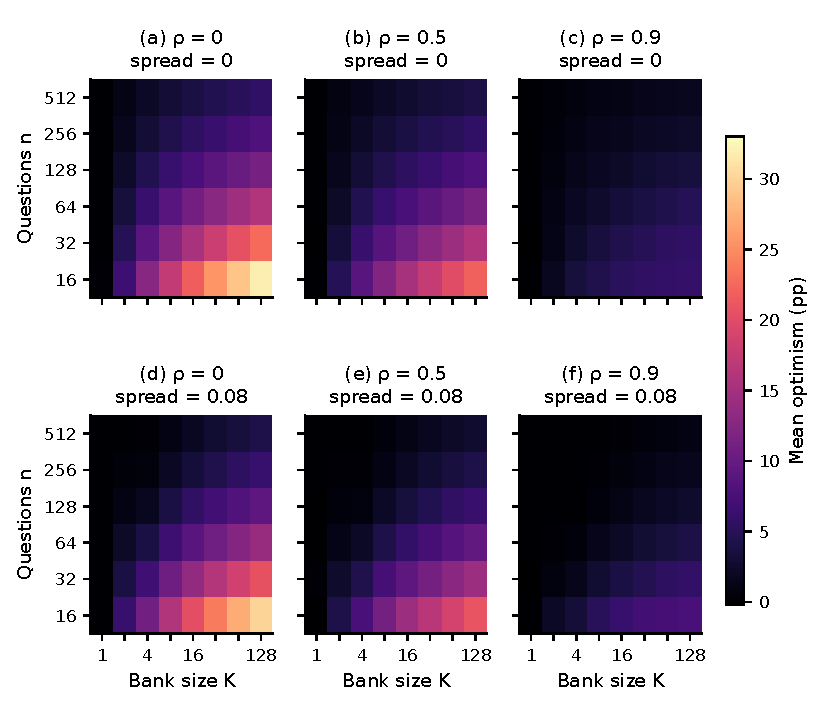
\includegraphics[width=\linewidth]{figures/synthetic-optimism-grid.pdf}
\caption{\textbf{Reused-score optimism in all 288 settings.} Color is mean winning search accuracy minus selected true accuracy, in percentage points. Rows vary quality spread, columns the shared-question mixture probability $\rho$; each panel crosses $n$ and $K$. At spread zero all accuracies are 0.4. At spread 0.08, nondefault means range over $[0.32,0.48]$; $K=2$ has a single 0.48 challenger, and $K=1$ only the default. Thus $K$ also changes the quality grid in heterogeneous cells. With unequal means $\rho$ is not exactly pairwise correctness correlation. The minimum estimate is $-0.176$ pp, reflecting Monte Carlo variation despite nonnegative expected optimism in this model. Complete per-cell MCSEs and seeds accompany the input CSV; this is not simultaneous inference about extrema.}
\end{figure}
\begin{figure}[htbp]
\centering
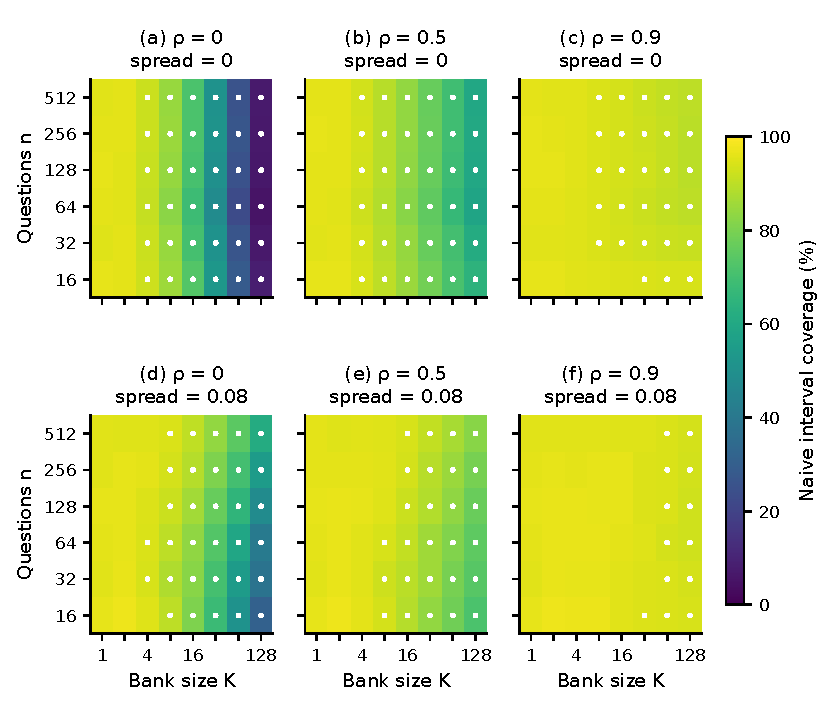
\includegraphics[width=\linewidth]{figures/synthetic-coverage-grid.pdf}
\caption{\textbf{Naive selected-target coverage in all 288 settings.} Settings match the optimism grid; color is the fraction of 20,000 repetitions where the ordinary nominal 95\% CP interval contains the selected candidate's known accuracy. A white dot marks a cell whose marginal exact 95\% Monte Carlo upper limit is below 95\%; these diagnostics are uncorrected across cells. Absence of a dot is not evidence of guaranteed coverage. Means, MCSEs, and seeds are retained in the complete source CSV.}
\end{figure}

\clearpage
\section{Point-estimation error}
\label{app:mse}
\begin{figure}[htbp]
\centering
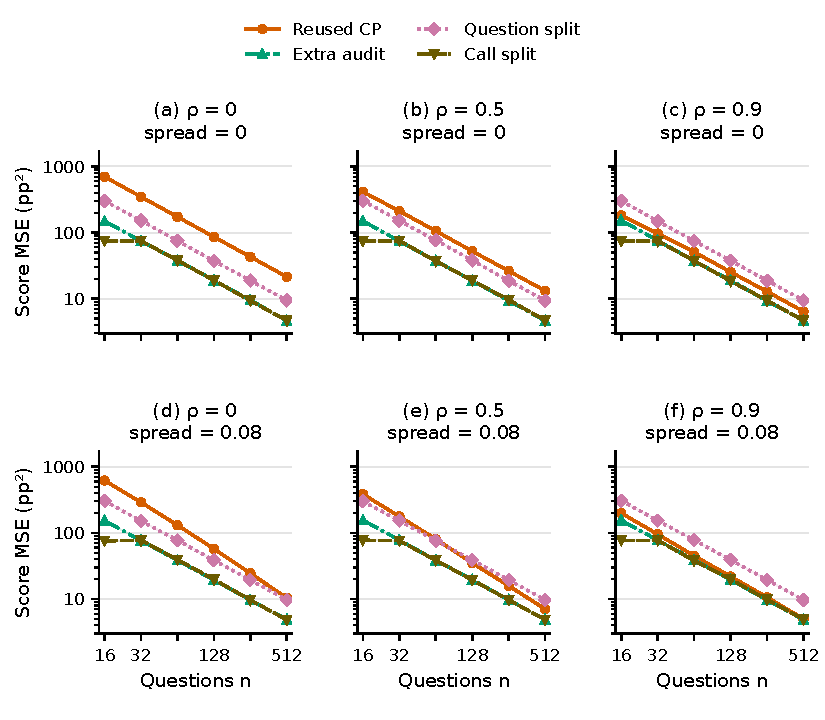
\includegraphics[width=\linewidth]{figures/synthetic-mse.pdf}
\caption{\textbf{MSE depends on protocol, resources, and candidate dependence.} At $K=32$, MSE averages squared error of a protocol's report relative to its selected true accuracy, in squared percentage points (log scale). Rows vary spread, columns shared-question mixture probability. Candidate means and resource definitions match the main figures. Simultaneous CP is omitted because it preserves the reused score and has identical MSE. Bands are mean $\pm1.96$ MCSE on the untransformed scale. Extra audit adds $n$ calls; question and call splits change selection resources and can select different configurations. These outcomes do not establish universal dominance or an actual LLM population effect.}
\end{figure}

\clearpage
\section{Numerical reporting and resource comparisons}
\begin{table}[htbp]
\caption{\textbf{Reporting protocols under two declared settings.} Entries are means (MCSE) from 20,000 independent repetitions. Bias is reported score minus the protocol's selected true accuracy. Width concerns nominal 95\% CP intervals; quality is the selected true accuracy. Bias and width are percentage points (pp), coverage and quality are percent. Both settings have $\rho=0.5$. Simultaneous CP retains the reused point score. Extra audit adds $n$ calls; question split preserves $n$ total questions; call split preserves $nK$ total calls. Parenthetical errors rounded to 0.000 are below 0.0005 in displayed units or exactly zero for constant truth. Full precision and counts accompany the source CSV.}
\label{tab:methods}
\centering
{\fontsize{8}{9}\selectfont\begin{tabular}{lrrrrr}
\toprule
Report & Bias (pp) & Coverage (\%) & Width (pp) & Quality (\%) & Calls \\
\midrule
\multicolumn{6}{l}{\textit{$n=64, K=16, \rho=0.5$; spread $0$}} \\
Reused CP & 7.71 (0.035) & 82.30 (0.270) & 25.39 (0.001) & 40.00 (0.000) & 1,024 \\
Simultaneous CP & 7.71 (0.035) & 98.29 (0.092) & 36.79 (0.002) & 40.00 (0.000) & 1,024 \\
Extra audit & 0.06 (0.043) & 95.84 (0.141) & 24.87 (0.005) & 40.00 (0.000) & 1,088 \\
Question split & -0.09 (0.062) & 95.25 (0.150) & 35.04 (0.010) & 40.00 (0.000) & 544 \\
Call split & 0.04 (0.043) & 96.03 (0.138) & 24.88 (0.005) & 40.00 (0.000) & 1,024 \\
\midrule
\multicolumn{6}{l}{\textit{$n=128, K=32, \rho=0.5$; spread $0.08$}} \\
Reused CP & 4.56 (0.027) & 88.33 (0.227) & 17.88 (0.001) & 46.52 (0.011) & 4,096 \\
Simultaneous CP & 4.56 (0.027) & 99.45 (0.052) & 28.03 (0.001) & 46.52 (0.011) & 4,096 \\
Extra audit & 0.01 (0.031) & 95.91 (0.140) & 17.81 (0.001) & 46.52 (0.011) & 4,224 \\
Question split & -0.04 (0.044) & 96.30 (0.134) & 25.24 (0.003) & 45.85 (0.016) & 2,112 \\
Call split & 0.04 (0.031) & 96.10 (0.137) & 17.81 (0.001) & 46.46 (0.012) & 4,096 \\
\bottomrule
\end{tabular}
}
\end{table}
\begin{figure}[t]
\centering
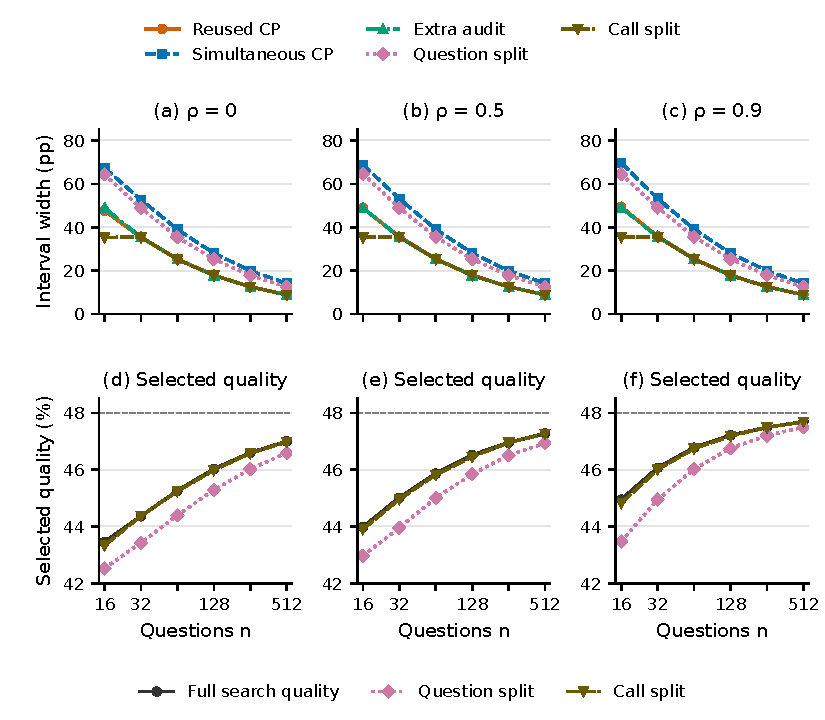
\includegraphics[width=\linewidth]{figures/synthetic-budgets.pdf}
\caption{\textbf{Reliable reporting trades uncertainty against search resources.} A bank of $K=32$ has a default accuracy 0.4 and other accuracies equally spaced over $[0.32,0.48]$. Columns vary shared-question mixture probability $\rho$, which is not exactly pairwise correlation for unequal means. Top: mean nominal 95\% interval width; bottom: mean selected true accuracy, with oracle 48\% dashed. Full search uses $nK$ calls. Extra audit adds $n$ calls and retains its winner. Question split reserves half the $n$ questions; call split uses $s=\lfloor nK/(K+1)\rfloor$ search and $h=nK-sK$ audit questions. Full-search methods share one quality curve. Bands are mean $\pm1.96$ MCSE over 20,000 repetitions. Width alone does not establish coverage, and split methods can select different targets.}
\label{fig:budgets}
\end{figure}
\clearpage
\section{Synthetic reproduction and compute}
The full grid was generated by \texttt{scripts/run\_synthetic.py} in the analysis package with \texttt{--reps 20000}, master seed 20261103, and independent cell seeds recorded in every output row. The exact-null reference script and distributional checks are delivered separately from the plotting code. Every synthetic figure and Table~\ref{tab:methods} is generated by \texttt{presentation/render.py} from hash-checked committed analysis inputs. The generator performs no simulation; it preserves upstream seeds and checks completeness and uniqueness of the metric grid. Each point-estimation band is mean $\pm1.96$ MCSE; event-rate bands use marginal exact binomial intervals, including nonzero upper limits for zero events.

The main synthetic run took 89.8811 measured computational wall seconds and 89.7073 process CPU seconds, with peak resident memory 285,564 KB. These timers exclude interpreter/import startup. The three-cell, 1,000-repetition pilot took 0.1761 wall seconds and 0.1614 process CPU seconds; its preliminary values are not substituted for full-grid results. No full-grid cells failed or were omitted. Plotting is documented separately by the presentation owner. The delivered reproduction instructions must also account for inference setup attempts and actual real-model generation; simulation timings are not total study costs.

\clearpage
\section{Real-model protocol, runtime fallback, and finite target}
\label{app:real-protocol}
This section records the executed protocol, runtime-driven scope revision, statistical guarantees and measured compute. Main findings are in Section~\ref{sec:real}. The original and derived manifests, pre-unblinding exposure hashes, raw outputs, complete analyses and execution records are supplied in \texttt{analysis/}.

\paragraph{Configurations and exposure.}
The study uses Qwen2.5-1.5B-Instruct with Q4\_K\_M quantization and CPU inference. The original eight candidates have frozen identities $[0,10,14,13,9,1,15,2]$, an outcome-independent prefix of a 16-member instruction/format bank. The fallback retains the first four, $[0,10,14,13]$; candidate 0 remains the default. Greedy direct-answer generation requests at most eight output tokens with context size 8,192. The strict capital-letter parser counts malformed and out-of-option answers as wrong, recording these failures and length endings separately. A complete valid answer at a length ending is not automatically incorrect. This differs from the original benchmark's random fallback after extraction failure. Only question and option text enter generation; gold answers and rationales do not. No main correctness or answer inspection informed the scope revision. The analysis owner preserves exact backend, model, prompt, parser, partition and code hashes, including the observed backend token-accounting anomaly.

\paragraph{Original design and runtime fallback.}
The pinned MMLU-Pro revision is \texttt{b189ec765aa7ed75c8acfea42df31fdae71f97be}. A uniform outcome-independent permutation assigns 512 test items to original search and 1,024 to original audit. Tier B would fill eight candidates on all 1,536 items, or 12,288 responses, in two sequential shards. The first shard evaluates even positions within each original pool and is complete: 256 search plus 512 audit items, with all eight candidates, totaling 6,144 generated answers. No second shard is required by the activated fallback. Retaining the first four candidates gives the primary Tier C matrix of 3,072 analyzed answers on 768 questions. The other 3,072 generated answers are preserved and costed but excluded from primary selection and calibration. No post-unblinding expansion is authorized.

The original stopping rule requires twofold remaining generation cost plus 48 hours of downstream reserve to fit the original one-week deadline, November 10, 2026 at 12:54:42 UTC. The analysis owner's completed-shard record reports 272,384.04 seconds (75.66 hours) of process elapsed time, 56,081.59 seconds (15.58 hours) of process CPU time, and 27,485.096 seconds (7.63 hours) of resource active wall time. These accounting boundaries differ; their discrepancy has not been attributed to suspension or model slowdown. Calendar elapsed cost triggers the already specified smaller design before main performance inspection. The earlier 11.8-hour nominal shard forecast was a planning extrapolation from validation, not an achieved elapsed time. Setup, pilots, failures, overhead and all generated responses remain in the cumulative accounting below.

\paragraph{Remaining-benchmark target and sampling.}
Let $B$ denote the pinned 12,032-item benchmark, $S_C$ the entire retained 256-item search reservoir, and $Y_j(x)$ the correctness of the frozen deterministic configuration $j$ on item $x$. The primary real target is
\begin{equation}
 \theta_{\rm rem}(j;S_C)=
 \frac{\sum_{x\in B\setminus S_C}Y_j(x)}{11{,}776}.
\end{equation}
Primary accuracy is question-weighted, not category-balanced. All smaller-$n$ search resampling retains the complement of the entire reservoir. The selected-minus-default contrast uses the same denominator and paired audit questions.

Under the fixed Tier C partition design, retained search, omitted search and retained audit occupy fixed disjoint positions in one uniform permutation. Conditional on the retained search identities, summing over the omitted original search identities leaves every retained audit set of size 512 equally likely in the 11,776-item complement. Thus the nominal fixed-design audit samples this complement without replacement. This argument does not condition on the original full 512-item search reservoir or on the runtime event selecting C. The audit is an estimate of remaining-benchmark accuracy, not known truth, full-benchmark accuracy or an unknown-question superpopulation mean.

\paragraph{Fixed-design intervals and runtime selection.}
For a fixed design with search size $s$, a candidate's search success count $x_j$ is hypergeometric under the uniform reservoir when its full-benchmark total is $M_j$. Inverting tails gives count endpoints $[L_j,U_j]$. Simultaneous bank protection uses per-candidate error $\alpha_d/K$. The map
\begin{equation}
 [L_j,U_j]\longmapsto
 \left[\frac{L_j-x_j}{12{,}032-s},
       \frac{U_j-x_j}{12{,}032-s}\right]\cap[0,1]
\end{equation}
preserves the simultaneous event and protects the selected remaining-benchmark target unconditionally over search reservoirs. Ordinary iid CP search intervals are comparators without this exact finite-design guarantee. For a fixed design, audit inversion instead has coverage conditional on the reservoir and search-frozen winner. A paired selected-minus-default contrast counts wins and losses on the same audit questions; hypergeometric intervals at error $\alpha_d/2$ for each count and subtraction of opposite endpoints conservatively protect their difference, without independent-category assumptions. Additional bank adjustment protects inspected nondefault contrasts.

Runtime may depend on question difficulty or response length even when correctness is not inspected. The supplied correction therefore allocates $\alpha_d=0.05/2=0.025$ to each of the two possible designs, B and C. Let $F_d$ denote a fixed-design failure event for one specified endpoint family. With arbitrary dependence between designs,
\begin{equation}
 \Pr(F_{D})\leq\Pr(F_B\cup F_C)
 \leq 0.025+0.025=0.05,
\end{equation}
where $D$ is the runtime-chosen design. This gives at least 95\% unconditional coverage over the original partition and tier choice. It does not establish coverage or audit unbiasedness conditional on the observed trigger. The adjustment protects the selected audit/gap, paired contrast and simultaneous bank/mixture endpoint families separately; all scientific endpoints are not jointly protected at 95\%. The nominal fixed-design conditional argument is not presented as a conditional guarantee after runtime selection.

\paragraph{Repeated selection and empirical-cache calibration.}
The retained grid uses $n\in\{16,32,64,128,256\}$ and $K\in\{1,2,4\}$, with 20,000 conditional selection repetitions. Whole paired rows preserve candidate dependence. Reuse of one audit pool means MCSE does not eliminate audit uncertainty. Simultaneous candidate audit intervals can bound a finite weighted mixture of selected accuracies when weights depend only on search, but that mixture is not automatically the infinite-repetition procedure expectation. The two-design adjustment also applies to the delivered bank/mixture endpoint family.

A separate 20,000-repetition experiment per cell samples iid paired rows with replacement from the 768-row retained response cache. Its exact candidate means are known. Repeating full selection and each reporting protocol permits calibration against this conditional empirical target using the original nominal 95\% iid methods. This does not establish coverage of remaining-benchmark or unknown future-question accuracy. An outer paired-row bootstrap of search and audit pools, with selection repeated, is a sensitivity analysis rather than an exact finite-population guarantee. The completed sensitivity run uses 1,000 outer and 2,000 inner repeats at $n=64,256$, $K=4$, after a timed pilot. It resamples each pool independently, preserving whole candidate vectors within questions, then repeats selection. Its 95\% percentile gap ranges are [5.45,18.46] pp at $n=64$ and [4.69,18.55] pp at $n=256$; paired-gain ranges are [5.26,11.65] and [5.46,11.91] pp. These approximate empirical ranges omit finite-population correction and retain inner Monte Carlo noise at $n=64$.

\paragraph{Logical reporting costs.}
For the retained design, selected-only auditing would require 512 additional calls; a paired winner-default audit requires 1,024 when identities differ. Filling the four retained audit columns uses 2,048 analyzed audit answers. The actual shard generated all eight audit columns, or 4,096 audit answers, plus 2,048 search answers. These logical reporting budgets and retained analysis counts must remain distinct from all 6,144 actual generated answers, their measured resource costs and setup/failure overhead. Reproduction preserves the original and derived manifests, raw caches, session/resource logs, seeds and exact commands rather than describing the fallback as a fresh experiment.


\paragraph{Prompts, seeds and diagnostics.}
The full sixteen-member bank crosses four instructions with four option delimiters, fixed before main outcomes. The retained prefix is $[0,10,14,13]$ (matrix columns are sorted IDs $[0,10,13,14]$). Default 0 asks, ``Solve the multiple-choice question. Respond with only the letter of the correct answer,'' using dot-separated options. Winner 10 asks, ``Read the question carefully and evaluate all answer choices. Output just the single letter identifying the correct choice,'' using colon-separated options. Candidate 14 uses ``You are taking a knowledge exam. Select the most accurate option. Your entire response must be its capital letter,'' with colons; candidate 13 uses the same instruction with parentheses. Literal rendered templates and the complete bank are in \texttt{analysis/provenance/prompt-bank.json} and the frozen runner. Uniform random tie breaking uses seed 20261109 for the primary winner, which is unique; conditional selection, cache calibration and bootstrap use seeds 20261107, 20261106 and 20261108. Each simulation output records its cell seed.

All 768 retained questions and their gold/scored outcomes are preserved; invalid responses are not dropped. The 398 malformed retained responses comprise 164 for default 0, 233 for candidate 13, one for candidate 14 and none for candidate 10. Parent-shard diagnostics record 1,094 malformed answers, no out-of-range letters and 727 length endings. The longest input has 1,143 tokens, below context size 8,192. Exact category and option-count denominators are in \texttt{analysis/results/real/data-diagnostics.json}; category accuracies are descriptive and do not alter the micro-accuracy target. Correlation/covariance exports identify both axes by actual candidate IDs. No category significance, causal dependence effect, parser repair or alternative post-unblinding extraction is claimed.

\paragraph{Cumulative compute and implementation failures.}
Inference used two CPU threads and no GPU, paid API or training, on an Intel Xeon Gold 6230 host subject to a two-CPU/4,096 MiB container ceiling. The native backend is \texttt{llama-cpp-python} 0.3.18, Python 3.11.2; source/compiler/environment and model/data hashes are delivered. Main generation used 1,424,801 prompt and 13,785 reported completion tokens, with peak resident memory 2,377,988 KiB. The two validation pilots add 114 responses; successful inference totals 6,258 responses, 1,448,117 prompt tokens and 14,001 completion tokens. Summed inference-session process CPU is 57,402.45 seconds, including startup/preflight. The native build separately took 301.917 resource-wall and 594.567 CPU seconds. These boundaries must not be conflated with the main elapsed/resource clocks above or with total study wall time.

Two prebuilt CPU wheels failed import because of an unavailable musl library; no answers came from them. Compiler acquisition initially failed certificate verification and succeeded with the configured certificate bundle, retaining verification. An interrupted model download was resumed and hash-checked. A validation output exceeded the requested eight-token cap while finishing a multibyte UTF-8 sequence; backend-source inspection records the relevant control flow. Accounting uses actual reported usage, and the cap is described as requested, without rewriting outputs. Exact records are in \texttt{analysis/provenance/failures.md} and \texttt{native-token-limit.json}.

The completed conditional-selection, empirical-cache calibration and bootstrap scripts measured 2.697, 1.971 and 36.471 computational wall seconds, respectively, excluding interpreter/import startup. The pilot measurements were 0.056, 0.156 and 0.095 seconds at their smaller declared sizes; these are not substituted for full results. Synthetic and plotting costs are separate. Numerical reproduction uses the committed matrix without additional LLM calls; rebuilding it from raw outputs requires the frozen parser's native dependency but loads no model. Exact acquisition, assembly, analysis and regeneration commands are in \texttt{analysis/docs/real-reproduction.md}. No second main shard was generated; the original larger design remains an abandoned generation plan in the provenance rather than a completed experiment.

\clearpage
\section{Complete real-model evidence}
\label{app:real-evidence}
All displays use the completed main run. Their generators, exact inputs and full-precision table CSVs are mapped in \texttt{presentation/real-output-map.json}.

\begin{table}[htbp]
\caption{\textbf{Reporting and uncertainty choices change the observed improvement decision.} Winner 10 is selected on 256 questions from $K=4$; audit 512 estimates accuracy on 11,776 questions outside that full reservoir. First three estimates/intervals are accuracy percentages; the final row is paired winner-minus-default accuracy in percentage points. Reused CP is the ordinary nominal 95\% binomial comparator, without an exact finite-benchmark/runtime guarantee. Exact search retains the reused point estimate and uses the transformed simultaneous finite-population interval. Disjoint audit and paired gain use exact finite-population intervals. These exact intervals allocate error .025 per possible B/C design and the exported within-design multiplicity; their at-least 95\% guarantee is unconditional after runtime choice, separately per endpoint family. The first three improvement entries use the exported conservative lower-winner-above-upper-default nonoverlap rule; the paired row instead asks whether its contrast lower bound is positive. Audit-supported improvement here is not a false-positive reuse decision. Calls (s) denotes logical uncached calls for selected accuracy alone; Calls (p) denotes calls for the improvement comparison, including a differing winner/default pair on audit. Reuse/search intervals cost 1,024 for either purpose. Disjoint auditing costs 1,536 for selected accuracy alone and 2,048 for the paired comparison. The paired gain has no selected-accuracy-only entry (dash). Actual generation cost is 6,144 main answers,3,072 analyzed and 3,072 retained but excluded, plus 114 validation calls and setup/failure overhead.}
\label{tab:real-reporting}
\centering
{\fontsize{8}{9}\selectfont\begin{tabular}{lrrrrr}
\toprule
Report & Estimate & Interval & Improvement & Calls (s) & Calls (p) \\
\midrule
Reused CP & 36.72 & [30.80, 42.95] & No & 1,024 & 1,024 \\
Exact search & 36.72 & [28.55, 45.46] & No & 1,024 & 1,024 \\
Disjoint audit & 25.39 & [21.27, 29.87] & Yes & 1,536 & 2,048 \\
Paired audit gain (pp) & 8.59 & [2.88, 14.14] & Yes & --- & 2,048 \\
\bottomrule
\end{tabular}
}
\end{table}

\clearpage

\begin{table}[htbp]
\caption{\textbf{Calibration, width, selection quality and cost are distinct reporting criteria.} Entries use 20,000 iid whole-row repetitions from the known 768-row empirical distribution at the declared setting $n=256$/$K=4$. Bias is report minus that protocol's selected candidate's true cache accuracy; bias/width are percentage points, coverage/quality percentages. Parentheses are MCSEs. Simultaneous CP retains the reused point score; reuse, simultaneous and extra audit share full-search quality. The extra audit uses 256 additional question draws; question split uses 128 selection/128 report draws, and call split uses 204 selection/208 report draws. Calls are hypothetical uncached totals 1,024/1,024/1,280/640/1,024, respectively, with no new inference during resampling. They differ from the primary disjoint audit 512 and actual 6,144 generated main answers. Width/quality MCSEs and exact selection/report counts accompany the full-precision table CSV. Displayed values rounded to 0.00 do not imply zero error.}
\label{tab:real-cache-methods}
\centering
{\fontsize{8}{9}\selectfont\begin{tabular}{lrrrrr}
\toprule
Report & Bias (pp) & Coverage (\%) & Width (pp) & Quality (\%) & Calls \\
\midrule
Reused CP & 0.21 (0.020) & 95.43 (0.148) & 11.46 & 29.02 & 1,024 \\
Simultaneous CP & 0.21 (0.020) & 98.91 (0.074) & 14.46 & 29.02 & 1,024 \\
Extra audit & -0.03 (0.020) & 95.51 (0.146) & 11.43 & 29.02 & 1,280 \\
Question split & -0.03 (0.029) & 96.60 (0.128) & 16.23 & 28.75 & 640 \\
Call split & -0.01 (0.022) & 96.15 (0.136) & 12.70 & 28.94 & 1,024 \\
\bottomrule
\end{tabular}
}
\end{table}

\begin{table}[htbp]
\caption{\textbf{Paired-row bootstrap sensitivity retains substantial question-pool uncertainty.} At $K=4$ and $n=64$/256, original means are from 20,000 conditional subset-selection repetitions; percentile ranges use 1,000 outer bootstrap draws with 2,000 inner selection repetitions each. Search and audit pools are independently resampled as paired candidate vectors, rerunning selection. Both the search-minus-audit gap and selected-minus-default audit gain are in percentage points. These are approximate 95\% empirical-bootstrap sensitivity ranges without finite-population correction or an exact/conditional-on-trigger coverage guarantee; inner MC error remains at $n=64$. They do not replace the exact runtime-protected primary intervals.}
\label{tab:real-bootstrap}
\centering
{\fontsize{8}{9}\selectfont\begin{tabular}{rlrr}
\toprule
Search n & Quantity (pp) & Original mean & Bootstrap 95\% range \\
\midrule
64 & Search minus audit & 11.55 & [5.45, 18.46] \\
64 & Paired audit gain & 8.45 & [5.26, 11.65] \\
256 & Search minus audit & 11.33 & [4.69, 18.55] \\
256 & Paired audit gain & 8.59 & [5.46, 11.91] \\
\bottomrule
\end{tabular}
}
\end{table}

\clearpage

\begin{figure}[htbp]
\centering
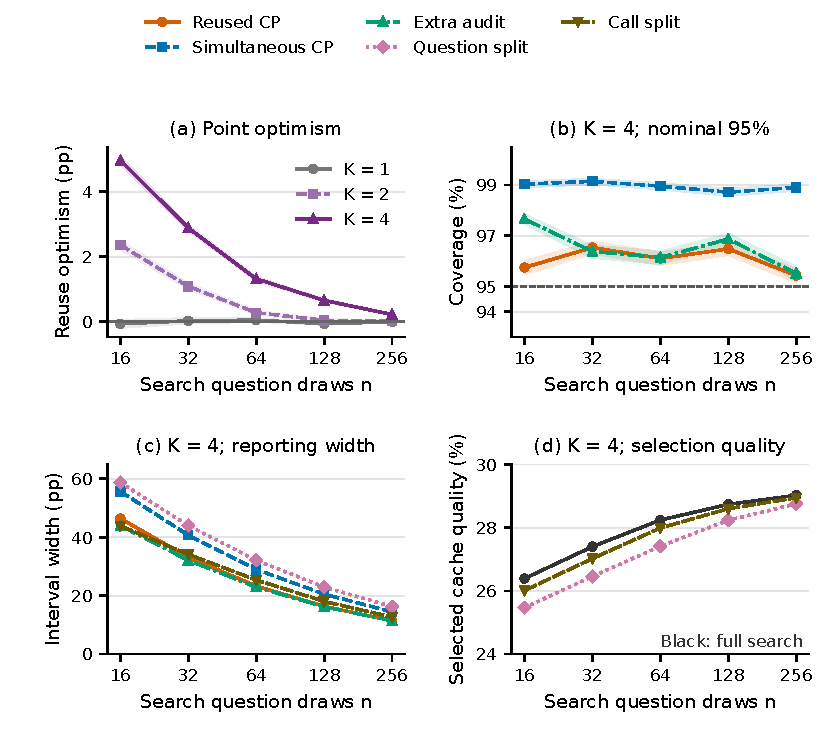
\includegraphics[width=\linewidth]{figures/real-cache.pdf}
\caption{\textbf{Positive point optimism occurs without observed nominal undercoverage in this small bank.} Conditional on the retained 768-row/four-candidate correctness cache, whole paired question rows are sampled iid with replacement, repeating full selection/reporting 20,000 times per n/K cell. The selected candidate's exact cache mean is the known target; it is distinct from remaining-benchmark accuracy. (a) Reused-score optimism for frozen-prefix K=1,2,4; adding candidates changes bank membership and true cache qualities. (b) Nominal 95\% selected-target CP coverage at $K=4$, with a dashed 95\% reference. (c) Mean interval width for all five reporting methods. (d) Selected cache quality for full search (black), equal-total-question-draw split and equal-total-call split. Reuse, simultaneous intervals and extra audit share the full-search winner. Bands are marginal 95\% Monte Carlo intervals: exact binomial intervals for coverage and mean$\pm$1.96 MCSE otherwise. They measure conditional computational error, not between-model or audit-pool uncertainty. At $K=4$, optimism declines from 4.97 pp at $n=16$ to 0.21 pp at $n=256$, while naive coverage across the entire 15-cell grid is 95.290--97.585\%. This setting does not reproduce the synthetic large-bank undercoverage. Simultaneous intervals retain the reused point estimate; the audit costs extra calls and splits can choose different candidates. The companion numerical table states budgets.}
\label{fig:real-cache-full}
\end{figure}
\clearpage
\begin{figure}[htbp]
\centering
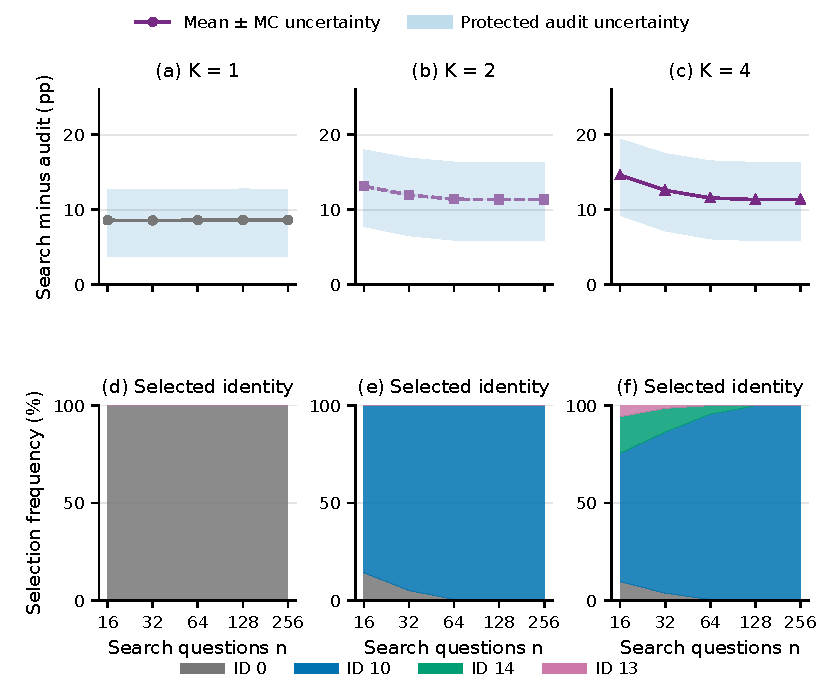
\includegraphics[width=\linewidth]{figures/real-conditional.pdf}
\caption{\textbf{The shared search--audit gap remains visible at $K=1$ and after repeated selection.} Columns use the frozen candidate-prefix sizes $K=1,2,4$; rows of the response matrix are kept paired across candidates. Top: mean selected search score minus audit score over 20,000 subset-selection repetitions at each n, conditional on one search/audit matrix. Narrow bands around curves are mean$\pm$1.96 conditional MCSE; blue regions are the analysis-exported bank-simultaneous, runtime-protected audit uncertainty bounds for the finite Monte Carlo mixture's true gap on the 11,776-item reservoir complement. These bounds retain audit uncertainty even when Monte Carlo error becomes small; they concern the finite Monte Carlo mixture rather than the infinite-repetition expectation. The displayed MC bands are marginal across cells. Each delivered endpoint family has at least 95\% unconditional protection over partition/runtime choice, with .025 error per design plus bank adjustment, and no conditional-on-trigger guarantee. Bottom: full-search winner frequencies over the same repetitions, with frozen identities labeled explicitly. All n use the complement of the entire retained 256-item search reservoir. Repetitions are computational reuse, not independent model runs or new audit datasets. Audit disagreement is not population false-superiority.}
\label{fig:real-conditional}
\end{figure}

\clearpage

\begin{figure}[htbp]
\centering
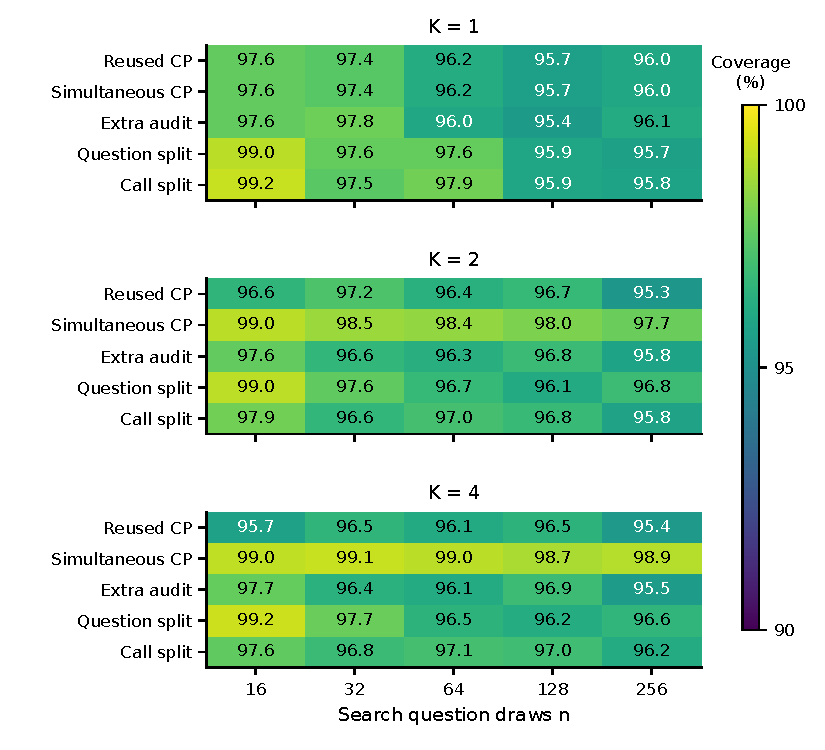
\includegraphics[width=\linewidth]{figures/real-cache-coverage-grid.pdf}
\caption{\textbf{Measured known-cache coverage remains above 95\% for naive reuse in all 15 tested cells.} Each panel fixes prefix K and displays nominal 95\% selected-target coverage for five reporting protocols across all five search sizes. Values are percentages rounded to one decimal; colors share a 90--100\% scale whose 95\% tick is the nominal reference. Each value uses 20,000 iid whole-row cache repetitions; exact 768-row empirical means supply truth. Point colors and rounded annotations omit MC intervals for space; full-precision means, MCSEs, seeds and repetition counts remain in the pinned input CSV. The main calibration figure displays marginal exact binomial MC bands, and the numerical comparison includes coverage MCSEs. Neither conservative coverage nor this small-bank null undercoverage finding establishes validity for the external audit or all prompt searches.}
\label{fig:real-cache-coverage-grid}
\end{figure}

\begin{table}[htbp]
\caption{\textbf{The conservative decision shows little false-claim activity in this cache.} Entries are event counts per 20,000 iid-cache repetitions, with reuse columns by K and the final column listing simultaneous counts for $K=1,2,4$ separately. A false event requires a selected nondefault winner's lower CP endpoint to exceed the default's upper endpoint when its exact empirical-cache quality is no better than the default. Reuse uses ordinary nominal 95\% CP endpoints; simultaneous uses .05/K marginal error. The only observed reuse event is at $n=32$/$K=4$; all simultaneous counts are zero. Zero of 20,000 still allows per-cell one-sided 95\% upper risk 0.000149775 (about 0.015\%), not zero risk or simultaneous protection across cells. The full-precision CSV includes marginal two-sided exact 95\% binomial MC intervals. This is conditional empirical-cache false-superiority, not a measured external-population error rate, paired test or claim-conditional false-discovery rate.}
\label{tab:real-cache-decisions}
\centering
{\fontsize{8}{9}\selectfont\begin{tabular}{rrrrr}
\toprule
Search n & Reuse K=1 & Reuse K=2 & Reuse K=4 & Sim K=1,2,4 \\
\midrule
16 & 0 & 0 & 0 & 0, 0, 0 \\
32 & 0 & 0 & 1 & 0, 0, 0 \\
64 & 0 & 0 & 0 & 0, 0, 0 \\
128 & 0 & 0 & 0 & 0, 0, 0 \\
256 & 0 & 0 & 0 & 0, 0, 0 \\
\bottomrule
\end{tabular}
}
\end{table}

\clearpage

\begin{figure}[htbp]
\centering
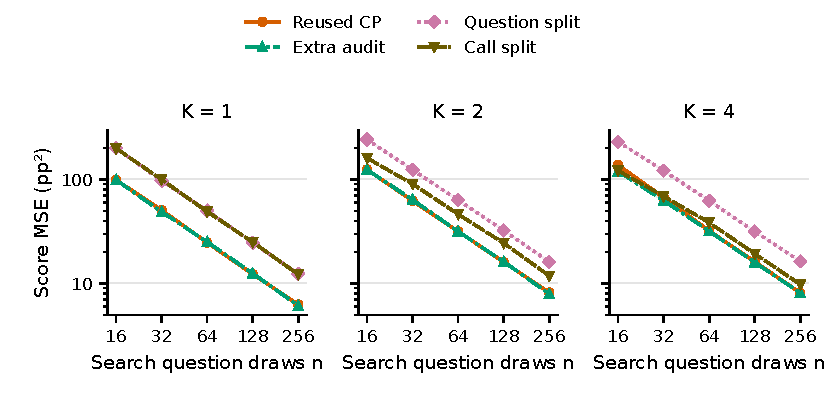
\includegraphics[width=\linewidth]{figures/real-cache-mse.pdf}
\caption{\textbf{Score error depends on reporting protocol and search size.} On the same 768-row empirical distribution, mean squared error is relative to each protocol's selected candidate's exact cache mean, in squared percentage points (log axis). Panels fix $K=1,2,4$ and retain all five n values. Bands are mean$\pm$1.96 MCSE over 20,000 iid-cache repetitions. Simultaneous CP is omitted because it preserves the reused point score and therefore has identical MSE. Extra audit uses n additional question draws/calls; question and call splits change selection sample sizes and may select different candidates. This is known-cache error, separate from squared differences against a noisy finite audit; no universal ranking or population-error claim is made.}
\label{fig:real-cache-mse}
\end{figure}

\begin{figure}[htbp]
\centering
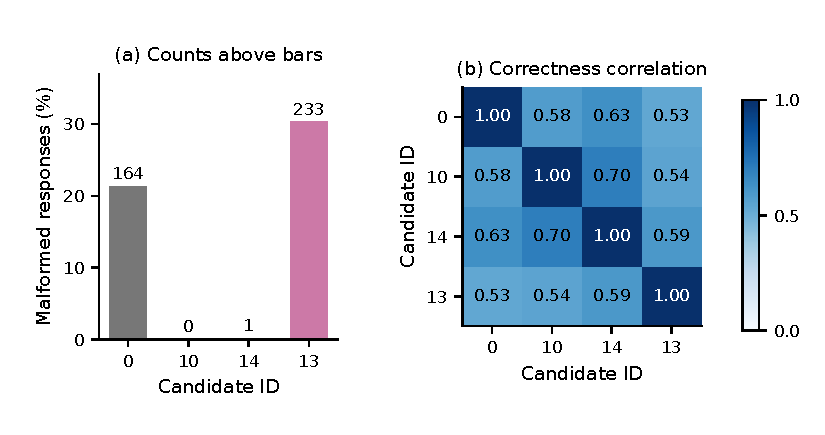
\includegraphics[width=\linewidth]{figures/real-diagnostics.pdf}
\caption{\textbf{The frozen prompt configurations differ in format adherence and share correctness patterns.} Left: malformed-output fraction for each retained candidate across 768 generated question responses; labels give counts, with a common 768 denominator. The strict frozen parser scores malformed answers wrong: default 0 has 164 malformed outputs, winner 10 none, ID 14 one and ID 13 has 233. These outcomes remain part of the tested system; no post-outcome parser repair was applied. Right: empirical correctness correlations across the same paired rows, with actual candidate IDs on both axes, a common 0--1 scale and values rounded to two decimals. These descriptive diagnostics do not establish a causal explanation of the gap or generalize across models. Full pool/category denominators and length-ending diagnostics are in the analysis package.}
\label{fig:real-diagnostics}
\end{figure}

\end{document}
